\capitulo{4}{Técnicas y herramientas}

\section{Kinetis}
Para conseguir almacenar los mensajes NMEA en la tarjeta microSD, se ha utilizado Kinetis Design Studio 3 IDE \cite{kinetis}. Se trata de un software de desarrollo basado en GNU/Eclipse antes utilizado en exclusiva para los servicios de los dispositivos de Freescale Kinetis. Desde la adquisición por parte de NXP ahora presta servicio a multitud de sistemas empotrados.

Soporta dispositivos Kinetis basados en Cortex-M, integra Processor Expert y un kit de desarrollo de software. 
Además soporta diversas herramientas de debugueo, entre ellas: SEGGER J-Link/J-Trace, P\&E USB Multilink Universal/USB Multilink Universal FX y CMSIS-DAP. Utiliza la nueva librería nano C que ayuda a reducir la memoria utilizada por el sistema embebido.

\section{Lenguaje C}
El lenguaje C \cite{C} es un lenguaje de programación poco tipificado, de tipo de datos estático y de medio nivel porque tiene las estructuras comunes de los de alto nivel, pero además también tiene estructuras que le habilitan un control a bajo nivel.

Cuenta como principal virtud la eficiencia que su código produce. Normalmente utilizado en la creación de software de sistemas y ciertas aplicaciones. La programación a bajo nivel permite la modificación de registros del procesador, lo que lo convierte en ideal para la programación de sistemas empotrados.

\section{Processor Expert}
Processor Expert \cite{ProcessorExpert} es un sistema de desarrollo para configurar, crear, optimizar y migrar componentes software para las placas de desarrollo. 
Los componentes embebidos propios de las placas de desarrollo, son módulos que puedes instalar con Processor Expert  y que vienen con una serie de funcionalidades incorporadas especialmente diseñadas para sacar el máximo partido a dicho componente. Cobra un papel muy importante en nuestro proyecto dado que la programación directa de sistemas empotrados es compleja. Se trata de una programación a muy bajo nivel que requiere el acceso y la modificación de registros o incluso llegando a la programación en ensamblador. Con la intención de evitar esto, nace esta herramienta que proporciona una serie de librerías que permiten la programación a más alto nivel.

Cuando lo usamos genera dependiendo del componente, cabeceras, ciertos archivos de configuración o código fuente.

Un componente representa un elemento hardware, un periférico, un algoritmo o cualquier colección lógica de funciones.
\begin{figure}[!h]
	\centering
	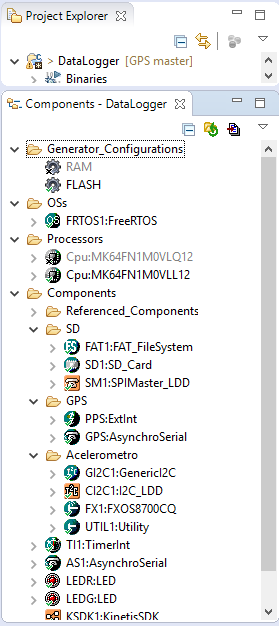
\includegraphics[width=0.5\textwidth]{ProcessorExpert.PNG}
	\caption{Processor Expert, vista de los diferentes componentes instalados.}\label{fig:ProcessorExpert.PNG}
\end{figure}
\FloatBarrier

\section{Termite}
Termite \cite{termite} es una terminal que permite la comunicación serie entre pc y placa, haciendo uso de los puertos COM del ordenador. Cuenta con una interfaz similar a la de un chat, en la que va mostrando toda la información que recibe y además cuenta con una línea para poder introducir texto y poder enviarlo.

\imagen{termite.PNG}{Terminal termite, ventana en blanco donde imprime la información que recibe.}

\section{Mapbox}
Mapbox \cite{mapbox} es un proveedor de mapas online para páginas web que nació en 2010. Se utiliza para integrar mapas en aplicaciones móviles y web.
Es una de las plataformas de datos más elegidas por los clientes por diferentes aspectos.
En Mapbox todo es personalizable, puedes escoger cualquier color, ocultar la capa que no quieras del mapa, etc. Tiene una serie de estilos predefinidos, pero también puedes crear el tuyo a través de la herramienta MapboxStudio.
Todo su código es open source y puedes encontrarlo en GitHub, lo que te permite ver las funcionalidades que están en desarrollo, notificar cualquier problema, hasta puedes contribuir mandando mejoras.
Se puede utilizar en cualquier plataforma, ya que hay SDKs disponibles para la mayoría, Android, iOS, web, etc.

\section{MyGeodata}
Mygeodata \cite{mygeodata} es un conversor de datos geográficos en línea que consta de diferentes formatos, CAD, GIS y Raster.

Se divide en tres apartados principales aunque en el proyecto solo se ha aprovechado el conversor:
\begin{itemize}
\tightlist
\item
	\textit{Drive}: en el cual puedes guardar tu conjunto de datos y gestionarlos o ver archivos que hayan compartido otros usuarios.
\item
	\textit{Converter}: es el apartado online donde puedes traducir tus coordenadas al formato de datos que elijas.
\item
	\textit{Map}: donde se muestran nuestros datos en un mapa de forma online.	
\end{itemize}

\section{XAMPP}
XAMPP \cite{xampp} es una herramienta que permite realizar pruebas de nuestro trabajo en el ordenador sin la necesidad de tener acceso a internet. Es una forma sencilla de instalar Apache.
Cuenta con un intérprete del lenguaje PHP, servidores de bases de datos como MySQL, servidores FTP, etc.
Su instalación es muy sencilla, basta con descargar y ejecutar un archivo comprimido, con unas pequeñas configuraciones. Además se actualiza de forma regular para que el usuario tenga las últimas versiones de los diferentes servidores que tiene.

\section{PHP}
PHP \cite{php} es un lenguaje \textit{open source} y puede ser incrustado en HTML.
Se ejecuta en el servidor web, por lo que puede tener acceso a bases de datos, conexiones de red y otra serie de tareas para crear la página resultado que será la que vea el cliente. Esta página final contendrá únicamente código HTML, por lo que será compatible con cualquier navegador.
Que el lenguaje se combine con HTML hace que sea fácil de utilizar, una de sus grandes ventajas, además de ser gratuito, multiplataforma, tenga una gran seguridad y rapidez.
Fue creado por Ramus Lerdorf en 1994, pero al ser de código abierto ha tenido varias contribuciones a lo largo de estos años.

\section{Python}
Python \cite{python} es un lenguaje orientado a objetos, que puede utilizarse para distintos objetivos, desde aplicaciones Windows a páginas web. Es muy conocido por varias razones, tiene una gran cantidad de librerías que cuentan con funciones muy útiles, es sencillo y rápido en comparación a otros lenguajes, se puede desarrollar en varias plataformas y es gratuito.
Fue creado por Guido Van Rossum, cuyo objetivo era un lenguaje que hiciese más fácil la orientación a objetos.
Las características más destacables del lenguaje son:
\begin{itemize}
\tightlist
\item
	Es de propósito general, puede utilizarse para la creación de varios programas.
\item
	Es multiplataforma, existen diferentes versiones para sistemas informáticos distintos.
\item
	Interpretado, no hay que compilar el código para realizar la ejecución. Es verdad que sí hay una compilación, pero es transparente al programador.
\item
	Es interactivo, podemos ejecutar cada sentencia para ver qué nos muestra.
\item
	Es un lenguaje orientado a objetos.
\item
	Cuenta con una gran cantidad de funciones y librerías que hacen más sencillo el trabajo, evitando tener que programar desde cero.
\item
	La sintaxis utilizada es muy sencilla y clara, se utiliza la tabulación para separar el código y distinguir los bucles o funciones.
	
\end{itemize}
Todo esto hace que Python actualmente esté siendo utilizado en empresas como Google, Yahoo, la NASA, etc

\section{GitHub}
GitHub \cite{GitHub} es una plataforma online de desarrollo colaborativo de software para almacenar en la nube proyectos, haciendo uso del sistema de control de versiones Git.
Git es un sistema de control de versiones de código abierto, gratuito y distribuido. Ha sido creado para poder manejar cualquier proyecto con eficiencia y velocidad. Github ha sido utilizado en este proyecto como piedra angular, para tener en todo momento el control sobre las distintas versiones.

\section{ZenHub}
ZenHub \cite{ZenHub} es una extensión que puede integrarse en GitHub, pero contiene interfaz propia.
Con ella nos ayudamos a tener un mayor control sobre nuestros proyectos, con un sistema de paneles, donde podemos ir catalogando las diferentes tareas según la fase de desarrollo en la que se encuentren. 

Los diferentes segmentos o \textit{pipelines} en los que se puede encontrar una tarea o \textit{issue} son: \textit{New issues, Icebox, Backlog, In progress Review/QA, Done y Closed} pero se pueden añadir más.

Además genera estadísticas, tiene un sistema de votación y permite obtener retroalimentación. Su gran baza al igual que GitHub, es que es gratuito para proyectos públicos. 

\section{LaTeX}
LaTeX \cite{latex} es un sistema utilizado para componer textos, principalmente indicado para aquellos que necesiten de una alta calidad de acabado tipográfico. Para la creación de esta memoria se ha utilizado Texmaker \cite{texmaker}.

\subsection{MiKTeX}
Además, junto con junto Texmaker hemos necesitado MiKTeX \cite{miktex} de código abierto, tiene compiladores LaTex y TeX y tiene la posibilidad de instalar unos 800 paquetes diferentes con macros, tipografías etc.

\section{Sonarcloud}
Sonarcloud\cite{sonarcloud} consiste en una plataforma \textit{online} que nos permite evaluar la calidad del código de nuestro proyecto de forma gratuita. Utiliza herramientas avanzadas que le permiten detectar posibles fallos o vulnerabilidades y que nos pueden ayudar a mejorar nuestro código. De forma general te presentan un panel informativo tras analizar el código con los siguientes aspectos: \textit{Bugs, vulnerabilities, code smells, coverage y duplications}. Se aporta el link del proyecto para poder revisarlo.

\section{Selenium}
Selenium\cite{selenium} es una herramienta que permite realizar pruebas de código sobre proyectos web. En nuestro caso se han llevado a cabo con Selenium IDE que ofrece una interfaz que permite grabar nuestros movimientos dentro de la web y provee una serie de comandos para hacer \textit{asserts} de una forma mas intuitiva que con Selenium WebDriver. De forma adicional permite exportar los test creados. 

